\section{Observational Constraints}\label{sec:observations}

\sgra is one of the most observed objects in the sky.  It has been observed with a slew of telescopes, across 5 decades in time and more than 17 decades in frequency. We need to select a manageable subset of this data to constrain our models. In doing so we have attempted to select
\emph{i})~approximately uncorrelated constraints, so that each tests a distinct aspect of the model;
\emph{ii})~constraints based on data that can be simulated with the models; and
\emph{iii})~constraints based on EHT 2017 1.3\mm VLBI data or based on photons produced within or close to the 1.3\mm emission region that are contemporaneous or near-contemporaneous.

Variability complicates the comparison of \sgra models to the data. Even an ideal evolution of a successful model will never match the data point for point because the space of possible realizations of the model is large; the dataset is high dimensional.  We expect the {\em distribution} of  observables derived from a successful model to match the data, however, if the model is run long enough to sample the distribution.  For example, the distribution of the 86\GHz flux density $F_{86}$ for a model ought to contain the observed $F_{86}$.

Most observables are correlated over $\tau\sim$ few $\times 100 \tg$.  To obtain the mean and variance of the model distribution to accuracy $f$ from a GRMHD model, then, requires running it for $\sim \tau/f^2 \sim 30,000 (\tau/300) (f/0.1)^{-2}$, assuming the model decorrelates completely at intervals $\gg \tau$.  A GRMHD model of duration $30,000 \tg$  costs $10^3-10^4$ node-hours, depending on resolution, code, and hardware.  This is expensive since $\sim 10$ runs are used for each model set, and runs need to be repeated for multiple values of numerical parameters (e.g. resolution).  Most of our models are run for $30,000 \tg$; a few are run to $100,000 \tg$.  The model distributions therefore contain sampling noise, and this must be accounted for in model selection.  For some  constraints (e.g. m-ring fits; see below) this can be done by sampling the model at a cadence similar to the correlation time and then using a 2-sample KS test to compare the observed and model distributions.

The constraints are heterogeneous and it is not possible to treat them completely consistently.  If a constraint returns a probability $p$ that, for example, the observed and model distributions are drawn from the same underlying distribution, then we reject at $p < p_c = 0.01$.  If a constraint returns a ``compliance fraction'' $f$ of, for example, the fraction of snapshots that are consistent with the data, then we also cut at $f < 0.01$.  For $N$ constraints a $p$ threshold implies that we expect to wrongly reject $1 - (1 - p_c)^N$ of acceptable models; for $p_c = 0.01$ and $N = 10$ this is $\approx 10\%$.

%==============================================================================
% \subsection{Scattering Models}

%==============================================================================
\subsection{EHT Observational Constraints}

%\ckc{ck's first pass}
%\mw{I think it would be good to mention the EHT array composition (name the telescopes)}
%\cfg{much of this material could be incorporated by reference to paperII}

% CFG: suggest we can do without these.  They do make what we are doing clearer, but it is yet another figure in a bazillion-figure paper.
%\begin{figure*}
%  \centering
%  \includegraphics[width=0.5\textwidth]{figures/va_comparison.pdf}%
%% \note{altex: (left) VA vs baseline for the day(s) that
 %   this study use, overplotted by the VA from a
%    fiducial model.
%    Similar to paper~II, figure~7.
%    Visually mark null location constraint, pre-imaging size (i.e.,
%    second moment).
 %   (right) SED from Gurther overplotted by the SEDs from a fiducial
%    model.
%    Visually mark the SED constraints.}
%  \caption{(\emph{left}) Measured correlated flux densities of \sgra
 %   on April 7, 2017, from the HOPS pipeline, overplotted with a fiducial
%    GRMHD+GRRT model.
%    Details on the data can be found in paper~II, section~5.
%    A description of the fiducial model is in section~\ref{sec:models}.
%    (\emph{right}) \ckc{Q: do we want to show only EHT observation and
 %     referencing to other papers for non-EHT constraints?
%      Or should we have representative figures for all measurements?}}
%  \label{fig:visibility}
%\end{figure*}

%The EHT observed \sgra at 1.3 mm during the 2017 April 5--11 observing campaign and obtained horizon scale complex visibilities.  Figure~\ref{fig:visibility} shows the VA on April 6 and 7 from  the HOPS pipeline, overplotted with VA derived from a model.  Evidently there are nulls near $\sim 5\,\mathrm{G}\lambda$ and $7\,\mathrm{G}\lambda$, suggesting a ringlike structure.

We test the models against EHT interferometric data in three ways.
First, we compare an estimate of the source size (``second moment'')
to an estimate from the short baseline visibility amplitudes (VAs).
Second, we check the location of the first minimum and the long
baselines values of the VAs (``\vam'').
Finally, using a variant of a procedure from \citetalias{PaperIV}, we
compare fits for the diameter, width, and asymmetry of an m-ring (a
parameterized image-plane model) to the GRMHD models.

%------------------------------------------------------------------------------
\subsubsection{230\GHz VLBI Pre-Image Size}
\label{sec:sz}

%% \ckc{ck's first pass}
%% \cfg{edited on 2 dec}
%% \ckc{I suggest we move the 2nd moment first, then null location, then
%%   m-ring.
%%   The reason is that the wide (unconstraining) 2nd moment is caused by
%%   allowing it to be just a Guassian (i.e., ignore the minima).
%%   We then tighten the constraint by regonizing there's a minima using
%%   the null analysis.
%%   And then do the fit.}

The source size can be characterized using the second moments of the
source image on the sky.
The second moments in the image domain map to second derivatives of
the visibilities near zero baseline in the $uv$ domain, so short
baseline VAs can be used to directly estimate the source size.

This procedure is used in \citetalias{PaperII} to set an upper limit
of 95\uas FWHM on the second moment and lower limit of 38\uas FWHM on
the second moment along a particular directions through the source,
with the direction determined by the orientation of the short
baselines.
This is done without any assumption about the structure of the source;
if we used a ring prior the constraint would be narrower.

%\cfg{is this scattered or unscattered?}
%\ckc{add descattered values}
The scattering kernel is estimated to have a 16.2\uas FWHM along the
relevant EHT baselines.
To descatter the sky image size, we subtract this value in quadrature
from the size.
This results an upper limit of 93.6\uas FWHM and lower limit of
34.4\uas FWHM.

To assess a model, we evaluate for each synthetic 230\GHz image the
second moment tensor and find its eigenvalues
$\lambda_\mathrm{maj}^2/(8\log 2)$ and $\lambda_\mathrm{min}^2/(8\log
2)$, where $\lambda_\mathrm{maj}$ and $\lambda_\mathrm{min}$ are the
FWHM of the major and minor axis.
The image is deemed non-compliant if it is inconsistent with the data for
all orientations, that is, if $\lambda_\mathrm{maj} < 34.4\uas$ or
$\lambda_\mathrm{min} > 93.6\uas$.
We reject models with a compliance fraction $< 0.01$.

%------------------------------------------------------------------------------
%\subsubsection{230\GHz VLBI Null Location}
\subsubsection{230\GHz VLBI Visibility Amplitude Morphology}

Our second constraint provides a simple morphological check on the
VAs.
We ask two questions of each model snapshot: \emph{i})~is the first
minimum in the visibilities in about the right place, and
\emph{ii})~are the long-baseline VAs comparable to the data?
For comparison, we use data from \aprilvii, which has the best $u$-$v$
coverage near minima in the VAs.

The minimum locations and long-baseline amplitudes are sensitive to the
source structure.
For example if the source is a simple, circularly symmetric ring of
finite width then the location of the first minimum depends only on
the ring diameter, while the VAs on long baselines depend mainly on
ring width.
GRMHD models are more complicated, with significant structural
fluctuations.
The minimum locations and depths, and long-baseline amplitudes, are
expected to fluctuate (e.g., \citealt{2018ApJ...856..163M},
\citetalias{M87PaperV}).

For the ``null location'', the first visibility minima in both the N-S
and E-W directions occurs between 2.5--3.5\,$\mathrm{G}\lambda$ in the
data \citetalias{PaperII}.
We do not consider the depth of the null in this simple check.

%% \cfg{best references for scattering?}
%% \ckc{add Dimitrios and Michael's papers}
For the ``long-baseline'' interval between 6--8\,$\mathrm{G}\lambda$,
the VAs have $\lesssim 4\%$ of the zero-baseline flux.
One complication when comparing models to data on long baselines is
the effect of interstellar scattering.
Diffractive scattering effectively convolves the image with a smooth
kernel and can reduce the amplitudes to about $\sim 50\%$ of their
unscattered values in the 6--8\,$\mathrm{G}\lambda$ range; refractive
scattering, on the other hand, introduces noise at all baselines of
order 0.5--3\%, depending on the particular characteristics of the
scattering screen \citep{2018arXiv180501242P, 2018ApJ...865..104J}.
To account for these effects, we classify a model snapshot with $|V|$
in this range that is $< 5\%$ of the zero baseline flux as compliant.

To apply this constraint, we compute the VA $V$ of each model snapshot
along position angles (PAs) $0^\degree$, $45^\degree$, $90^\degree$,
$135^\degree$.
Because of Hermitian symmetry this actually covers eight PAs.
We find the first minimum numerically and compute the median VAs
between 6 and 8\,$\mathrm{G}\lambda$.
We classify a snapshot as compliant if
\emph{i})~for at least one position angle the first minimum falls
between 2.5 and 3.5\,$\mathrm{G}\lambda$ and
\emph{ii})~at no position angle do the median VAs exceed $4\% /
50\%$ of the zero-baseline flux.
\michi{Does this mean 4\% < VA < 50\%? Then I would rephrase: "at no position angle do the VAs fall outside the range 4\%--50\%" Otherwise I don't understand this sentence.}
%See also Figure~\ref{fig:sample_va} and its caption.

We evaluate the fraction of snapshots from each model that are
compliant using the criteria described above.
We reject models with compliance fraction $< 1\%$.

%------------------------------------------------------------------------------
\subsubsection{230\GHz M-Ring Fitting}

How can we extract information about the spatial structure of the source from noisy, fluctuating data with limited UV coverage, and compare that to noisy, fluctuating models?
Our strategy is to fit a source-plane model to the data and summarize the source structure using the distribution of fit parameters.

\citetalias{PaperIV} fits an ``m-ring'' source model to the April~7 data.  Here we use a simplified m-ring model: a $\delta$ function in radius with diameter $d$ multiplied by a truncated (up to $m = 3$; Paper IV truncates at $m = 4$) Fourier series, convolved with a Gaussian of width $w$.  In addition the model contains a centered Gaussian component, with amplitude and width as free parameters, to absorb large scale emission and emission interior to the ring.

The simplified m-ring model has 10 parameters; 3 well constrained and physically interpretable parameters are used here: the m-ring diameter $d$, the m-ring width $w$ (FWHM of the convolving  Gaussian), and the $m=1$ relative amplitude $\beta_1$ (the ``asymmetry'').

We fit the m-ring independently to ``snapshots'' consisting of 2-minute intervals of EHT data. Over these short intervals, we approximate the source to be static.  Uncertainties in the fitted m-ring parameters are dominated by the limited baseline coverage during these snapshots rather than by calibration uncertainties or thermal noise. Because snapshots that are close in time sample nearly identical baselines, they do not provide additional model constraints.

Thus, to compare fitted m-ring parameters from the EHT data to those for synthetic data from simulations, we focus on a reduced comparison dataset that consists of only a subset of scans with the best baseline coverage. We select scans that are widely separated in time, so that they sample distinct baseline coverage. For the comparison dataset we selected ten 120-\sec scans spread approximately uniformly through EHT observations on \aprilvii.  They are separated by an average of $\simeq 1240\sec \simeq 60 \tg$, which is small compared to the VA correlation time in the models (see Georgiev et al. 2022). The scans were selected to have > 10 baselines, and integration time at all stations $> 40s$.  Only modest changes in model selection were observed if any one scan was removed from the comparison.  The data were de-scattered before fitting, that is, the VA were divided by the scattering kernel.  Maximum likelihood m-ring parameters were found for each scan.

The maximum likelihood m-ring parameters are listed in Table~\ref{tab:mringfits}.  Evidently the fit parameters are noisy.  The fit for $d$ range from 39\uas to 84\uas, for $w$ from 9\uas to 21\uas, and for $\beta_1$ from $0.04$ to $0.48$ (we require $\beta_1 \le 0.5$ to guarantee  positivity of the model image).

\begin{deluxetable}{ccccc}
  %
  \tablehead{ %
    \colhead{Scan \#} & %
    \colhead{t [UTC hrs]} & %
    \colhead{d [$\mu$as]} & %
    \colhead{w [$\mu$as] } & %
    \colhead{$\beta_1$} %
  }
  \startdata
  111 & 11.28 & 83.87 & 8.87  & 0.122 \\
  121 & 11.78 & 57.09 & 13.98 & 0.220 \\
  125 & 11.92 & 55.63 & 16.46 & 0.132 \\
  130 & 12.35 & 40.68 & 19.08 & 0.039 \\
  134 & 12.62 & 57.22 & 17.22 & 0.368 \\
  142 & 12.92 & 58.80 & 17.55 & 0.208 \\
  149 & 13.28 & 52.31 & 21.16 & 0.278 \\
  155 & 13.75 & 38.94 & 18.17 & 0.482 \\
  163 & 14.05 & 56.22 & 19.86 & 0.470 \\
  171 & 14.38 & 39.48 & 17.71 & 0.408 \\
  \enddata
  %
  \caption{M-Ring Fits to EHT Observations}
  \label{tab:mringfits}
\end{deluxetable}

The variation in fit parameters could be caused by source variability, thermal noise, and gain variations.  In the models the main driver of fit variations is source variability.

Next, we read in a series of model images, generate synthetic data for each image for each scan at four assumed position angles for the image, and fit m-rings to the synthetic data.  This produces a distribution of m-ring parameters for each model.

The synthetic data is generated as follows.  A model image $I(x,y)$ is Fourier transformed to complex visibilities $V(u,v)$ with an assumed position angle, then sampled on baselines $i$ drawn from the comparison scan, $V_i \equiv V(u_i,v_i)$.  Normally distributed thermal noise $\delta V_{th,i}$ with amplitude based on telescope performance during the scan is added, and multiplicative, normally distributed noise with unit variance $N$ is added to crudely model gain corrections: $\tilde{V}_i = V_i (1 + \epsilon N) + \delta V_{th,i}$.  We set $\epsilon = 0.05$, but no significant changes in fit parameters were observed for $\epsilon = 0.02$.  We then fit to the VA $|\tilde{V}_i|$ and closure phases.
%arg$(\tilde{V}_i \tilde{V}_j \tilde{V}_k^*)$, where $ijk$ form a triangle in the $(u,v)$ plane.
The procedure was repeated for 4 positions angles (orientations of the image on the sky) and for model images separated by $500 \tg$ (comparable to a correlation time; no significant changes were observed if more position angles were used).  This results in, for example, a sample of $30$ fits per scan per position angle for the Illinois thermal model set, or a total of $30 \times 10 = 300$ samples in each distribution.

In comparing the models to the data we
\emph{i}) generate the distribution of fit parameters at each position angle;
\emph{ii}) use a Kolmogorov-Smirnov test to compare the distribution of $300$ synthetic data fits with the distribution of $10$ observational fits, and obtain a p-value (what is the probability they are drawn from the same underlying distribution?);
\emph{iii}) average p-values over position angles (i.e. marginalize over position angle; the models do not show a significant position angle preference); and
\emph{iv}) reject the model if $p < 0.01$.

%==============================================================================
\subsection{Non-EHT Constraints}

In addition to the EHT data, the SED of \sgra is well constrained \citetalias{PaperII} and thus potentially useful for model selection.
We limit comparison to three bands: 86\GHz, 2.2\um, and x-ray, which are relatively independent and allow us to probe different physics.

%------------------------------------------------------------------------------
\subsubsection{86\GHz Flux}

The Global Millimeter VLBI Array (GMVA) observed \sgra on April 3, 2017, just 3 days ($\approx 13,000 \tg$) before the EHT campaign.
\citet{2019ApJ...871...30I} estimate that the compact flux is $F_{86} = 2.0 \pm 0.2\,\mathrm{Jy}$ ($2\sigma$ errors; S. Issaoun, private communication).

We compute a library of 86\GHz images for all GRMHD snapshots for all models, and from that the 86\GHz flux density $F_{86}$.  We assume normally distributed measurement errors with $\sigma = 0.1\,\mathrm{Jy}$, and convolve the $F_{86}$ distribution for each model with the resulting Gaussian.  We reject models with CDF $< 1\%$ or $> 99\%$ at $2.0\,\mathrm{Jy}$.

%------------------------------------------------------------------------------
\subsubsection{86\GHz Image Size}

The GMVA observations from April 3, 2017 constrain the FWHM of the source major axis ${\rm FWHM}_{maj} = 146^{+11}_{-12}\uas$ \citep[95\% confidence][]{2021ApJ...915...99I}.

We compute the major axis FWHM for each image in the 86\GHz image library.  We assume normally distributed errors with $\sigma = 6\uas$, and convolve the model major axis distribution with the normal distribution.  We reject models with CDF $< 1\%$ or $> 99\%$ at $146\uas$.

Our synthetic 86\GHz images have a 800\uas field of view.  A 200\uas field of view cuts off enough emission that the major axis is biased downward in many models by $\sim 20\%$.  Increasing the field of view beyond 800\uas has negligible effect.

%------------------------------------------------------------------------------
\subsubsection{NIR (Non-Overproduction) Constraints}\label{subsec:nir}

\sgra flares in the near infrared (NIR; 2.2\um) a few times per day (1 day $\simeq 4200 \tg$) \citep{2018ApJ...863...15W}, and has a quiescent flux that was estimated to be $\simeq 1.0\,\mathrm{mJy}$ in 2017 \citep{2020A&A...638A...2G}.  Since there is as yet no generally accepted model for NIR flares, we accept models that do not produce flares.  Our working hypothesis is that these models can be saved by perturbatively introducing a process that accelerates a small fraction of electrons into a nonthermal, NIR-bright tail.  If the model overproduces NIR with just the thermal electron population then we reject it.

We compute the 2.2\um flux density using one of two procedures.  If a full SED\textemdash which includes Compton scattering\textemdash is available, then it is used. The SEDs are generated by the \grmonty Monte Carlo code \citep{2009ApJS..184..387D, Wong_2022, Davelaar_2022}. If a full SED is not available then we compute a NIR image that includes only synchrotron emission and absorption (although synchrotron absorption is negligible in the NIR for \sgra).  We reject the model if the median NIR flux density exceeds $1.0\,\mathrm{mJy}$.

%------------------------------------------------------------------------------
\subsubsection{X-ray (Non-Overproduction) Constraints}

\sgra flares in the x-ray less than about once per day \citep[see, e.g.,][and reference therein]{2018MNRAS.473..306Y}.  Chandra observations during the 2017 campaign suggest an upper limit on the median (quiescent) $\nu L_\nu$ at $6\,\mathrm{keV}$ of $10^{33}\ergsps$ \citep{PaperIII}.

Similar to section \ref{subsec:nir}, we estimate $\nu L_\nu(6\,\mathrm{keV})$ in two ways.  The SED is used if the model contains Compton scattering and bremsstrahlung.  If the SED is not available then we compute an x-ray image that includes only bremsstrahlung (which dominates the x-ray emission in thermal SANE models with $\Rh = 40$, $160$) permitting us to eliminate a few additional models.  We reject the model if the median $\nu L_\nu(6\,\mathrm{keV}) > 10^{33}\ergsps$.

%==============================================================================
\subsection{Variability}

% * we can model ``long-term climate'' well but not ``long-term weather''.
% * Hence we only compare the slowly varying quantities such as mean/median 2nd moments (climate) but not modulation index (weather).
% * TODO: look up correct statistical terminology in weather/climate modeling and build that this into this paper.
% * Use review: https://agupubs.onlinelibrary.wiley.com/doi/full/10.1029/2019EA000586 , https://ui.adsabs.harvard.edu/abs/1993RvMP...65.1331A/abstract
%
% * multi-time scale
% * feeding at large and slow scale
% * time scale much shorter when the plasma reach horizon
% * at 1.3mm, we only see the flow near the horizon
% * a "hidden variable" problem that there're slowly varying "boundary conditions" that control the nature of the accretion flow
% * but we only see the fast varying flow
% * Given the boundary conditions (environment), GRMHD + GRRT is very successfully in predicting the time average images.  (Refer to consistent checks in appendex)
% * At the short time scale, the system is chaotic and sensittive to initial conditions.
% * We reach order-of-magnitude agreement.  But in terms of constraint they should not be used.
% * For the date we use, EHT observations show lower variability compared to what we expected.

%\cfg{I think we should just describe the observations here.}
%\ckc{We don't have a discussion section on variability yet.  Maybe under 5.7 or 5.8?}

\sgra shows variability on a wide range of timescales.  This is expected: fluctuations in stellar wind feeding at the scale of the S-stars plausibly introduce long timescale variations, while turbulence at smaller radii, down to the scale of the event horizon, plausibly introduce a spectrum of shorter timescale variations.  Quantitative comparison of observed variability to the models is therefore a potentially powerful tool for model selection.

Here we consider two measures of variability: one that characterizes variability of 230\GHz flux density in the light curves \citep{Wielgus2022} and a second that characterizes variability of the VA in EHT data \citep{PaperIV, NoiseModeling}.

\cfg{are these numbers still correct?}
\michi{For all models 66.5\% fail MI. For Illinois/Frankfurt thermal, 76\% fail MI.}
We will find that $> 90\%$ of models fail the combined variability tests: the data is quieter than the models.  This is the most severe downselect of all our constraints. Given the noisy nature of the model selection process we do not interpret this as success for the surviving $10\%$, all of which fail other constraints.  Instead we interpret this as a particular and interesting failure of the entire class of GRMHD models to reproduce the observed variability.  We discuss possible reasons for this {\em variability crisis} in Section~\ref{sec:discussions}.

%The remaining non-variability constraints are still informative about the structure of \sgra.  We therefore set aside the variability tests and perform a final model selection considering only the remaining constraints.  This is a dangerous game in the sense that variability is deeply embedded in many of the remaining constraints (it determines the width of many of the model distributions that we use for selection, for example).  Still, it is remarkable that so many models look as much like the data as they do, and rather than set aside that information we use it to identify a final set of best-bet models.

%Although we provide a full discussion of model variability, we will not use it for model selection, under the notion that the variability is a higher-order - and therefore less well predicted -  feature of the models while lower order features, such as 86\GHz flux density and 230\GHz source geometry, are still well predicted.  This hypothesis can only be tested once models that accurately predicted variability are available.

%Compared to other astrophysical systems, optically thin black hole accretion systems such as \sgra are expected to show variabilities in a wide range of time scales, from the boundary conditions at the Bondi radius determined by the ``environment'', all the way to the turbulent fluctuations near the event horizon, or even plasma instability driven phenomena.
%Even excluding flares and detailed plasma physics, observations have shown intrinsic variability in \sgra~\citep{sgra lightcurve papers}.
%The standard theoretical interpretation is that the turbulence in the accretion flow drives the fluctuations in, e.g., temperature and magnetic fields, which then drive the fluctuations in the electromagnetic signals.
%Assuming that the magnetorotational instability (MRI) is the driving mechanism, the turbulence integrated time scale is simply the orbital time scale.
%Given that synchrotron radiation mainly comes from the inner accretion disk, this time scale is of order of 10 minutes.
%However, the chaotic nature of turbulence makes these short time scale variability difficult to predict.
%Therefore, we will not rule out models using short time scale variability.
%On the other hand, numerical simulations are very successful in predicting the slowly varying mean images, SEDs, etc because these are controlled by the conservation laws and the boundary conditions.
%This justifies the usage of mean and median quantities to constraint models described in the earlier sections.

%------------------------------------------------------------------------------
\subsubsection{ALMA Light curves}

%\mw{I edited this a bit}
% thanks Maciek -CG

ALMA and SMA produced \sgra light curves at 230\GHz as a byproduct of the 2017 EHT VLBI observing campaign. The complete set of light curves is presented and analyzed in \cite{Wielgus2022}.

We have chosen to compare the models to light curve observations of \sgra from 2005-2017 using the 3 hour {\em modulation index} $\mi{3}$, where $\mi{T} \equiv \sigma_T/\mu_T$, $\sigma_T$ is the standard deviation measured over some interval $T$, and $\mu_T$ is the mean measured over the same interval.  We use $\mi{T}$ following \citet{2015ApJ...812..103C} because it is easy to describe, easy to compute, commonly used in the literature (in the x-ray astronomy literature it is ``rms \%''), and closely related to the structure function, since the expectation value for $\sigma_T^2$ is given by an integral over the structure function \citep[see][]{Lee_2022}.

We use $T = 3$ hours because it is comparable to the correlation time for $F_{230}$ in most of the models, and because it is similar to the characteristic timescales measured in damped random walk fits to the ALMA light curve \citep[see Table 10 of][]{Wielgus2022}.  Although the correlation times tend to be slightly longer than 3 hours, that is the longest timescale for which we can consistently estimate the mean and variance of the distribution of $\mi{3}$ from the models (accurate estimation for larger $T$ would require longer GRMHD integration times).  In a damped random walk process one can show that $\mi{3}$ is minimally correlated over consecutive 3 hour intervals \citep{Lee_2022}.

For each light curve, we take 3 hour segments equally spaced away from the endpoints and each other, and calculate the $\mi{3}$ on each segment. This gives us a set of 42 samples of the $\mi{3}$ for the historical dataset. We note that the $\mi{3}$ measured from the EHT 2017 observations on April 5-11 are consistent with being drawn from this distribution, although April 7 has one of the quietest segments on record, while April 11 has one of the most variable.

% old version, revised out following D. Lee 11-dec cfg
%We have chosen to compare the models to the 7 April 2017 ALMA light using the 3 hour {\em modulation index} $\mi{3}$, where $\mi{T} \equiv \sigma_T/\mu_T$, $\sigma_T$ is the standard deviation measured over some interval $T$, and $\mu_T$ is the mean measured over the same interval.  We use $\mi{T}$ following \citet{2015ApJ...812..103C} because it is easy to describe, easy to compute, commonly used in the literature (in the x-ray astronomy literature it is ``rms \%''), and closely related to the structure function, since the expectation value for $\sigma_T^2$ is given by an integral over the structure function (see Lee et al. 2022).

%We use $T = 3$ hours because it is comparable to the correlation time for $F_{230}$ in most of the models, and because it is similar to the characteristic timescales measured in damped random walk fits to the ALMA lightcurve \citep[see Table 10 of][]{Wielgus2022}.  Although the correlation times tend to be slightly longer than $3$hr, that is the longest timescale for which we can consistently estimate the mean and variance of the distribution of $\mi{3}$ from the models (accurate estimation for larger $T$ would require longer GRMHD integration times).  In a damped random walk process one can show that $\mi{3}$ is minimally correlated over consecutive 3 hour intervals (Lee et al. 2022).

%We measure $\mi{3}$ in maximally spaced intervals in the ALMA lightcurve on April 6, 7, and 11.\footnote{The model comparisons are insensitive to interval spacing.}  We have also measured $\mi{3}$ in historical data for \sgra from 2005-2017 light curves.  The April 6, 7, and 11 values for $\mi{3}$ (5 in all: 0.029, 0.031, 0.051, 0.041, 0.099) are consistent with having been drawn from the historical distribution, although April 7 is among the quietest intervals on record and April 11 is one of the most variable intervals on record.

For each model we evaluate a light curve and use that to generate a distribution of $\mi{3}$.  We then use a KS test to ask whether that distribution is consistent with the historical distribution.
%The constraint comes from $M_T$ measured over 3 maximally spaced intervals
%in the 7 April 2017 ALMA light curve, where $M_3 = 0.024, 0.051,
%0.047$ (Wielgus et al. 2021). These values are consistent with being drawn from the distribution estimated from historical non-EHT 2005-2017 light curves.
%curves. \mw{maybe sth like "from the estimated distribution of the historical 2005-2017 lightcurves"?}

%%%%%%%%%%%%%%%%%%%%%%%%%%%%%%%%%%%%%%%%%%%%%%%%%%%%%%%%%%%%%%%%%%%%%%%%%%%%%%%
% This figure is for the Standard Models:EHT Constraints:Second Moment section
\begin{figure*}
  \centering
  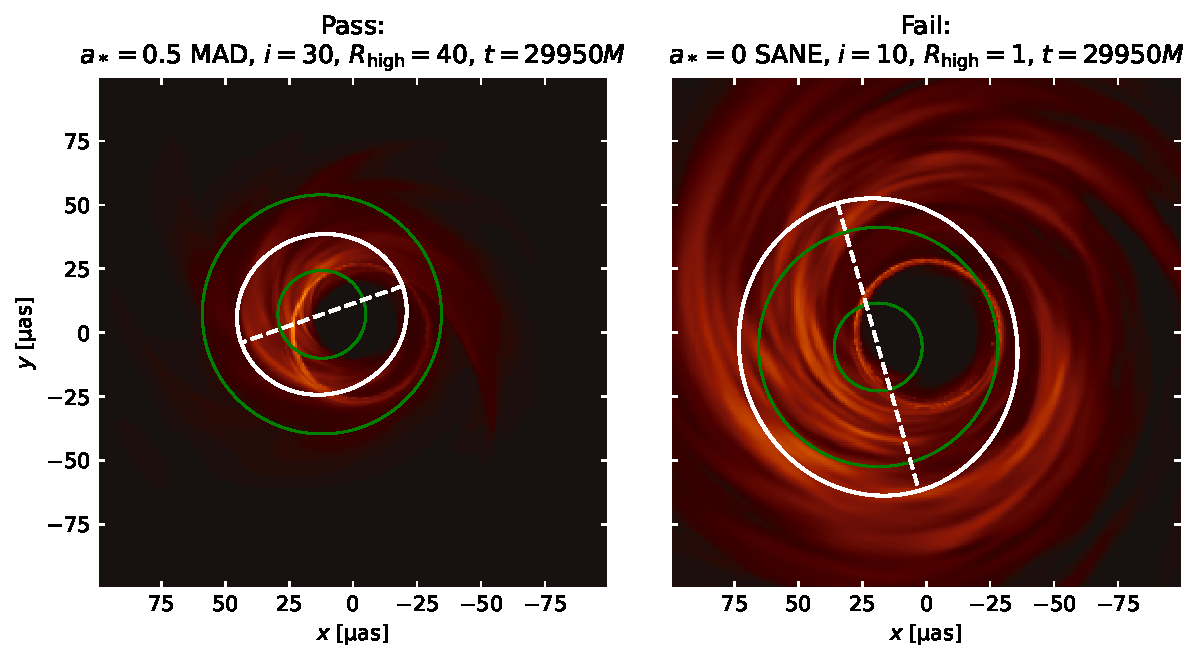
\includegraphics[width=0.75\textwidth]{figures/passfail_sz.pdf}
  \caption{Second moment constraint example.  Left: passing snapshot; right: failing snapshot.  The model is rejected if $< 1\%$ of model snapshots pass.  Solid white ellipse  represents the second moments of the image, and the dashed line shows the major axis.  The two green circles show the observed lower and upper limits from \cite{PaperIII}. The snapshot is rejected if either the major or minor axis lies between the lower and upper limits. 
  % cfg 15-dec: edited down
  %Visual representation on how the second moment constraint work. For each of the panels, the white ellipse represents the FWHM of the Gaussian fits. Hence, the white dashed shows the FWHM major axes, and an invisible line perpendicular to that is the FWHM minor axes. The two green circles mark the upper and lower limits of the allowed size. Given the relax criteria described in Section~\ref{sec:sz}, an image is deemed compliant as long as the white ellipse touch the region between the two green circle. The left panel is a feature model (see Section~\ref{sec:bestbets}) that passes this constraint because the white ellipse falls between the two green circle. The right panel is zero spin SANE model with $i=10$ and $\Rh = 1$, that fails this constraint because even its minor axis is too big compare to the upper observed limit.
  }
  \label{fig:passfail_sz}
\end{figure*}

%------------------------------------------------------------------------------
\subsubsection{EHT Structural Variability}

%\ckc{I think Boris needs to write this...}

%Fluctuations in source structure will lead to fluctuations in VA. \citealt{NoiseModeling} describes a technique to measure the variance of the spatially-debiased VA at a location in the $(u,v)$-plane. Due to the sparse coverage of the 2017 EHT observations, this variance is calculated over the first four days (April 5, 6, 7, 10), and azimuthally averaged. Using the contemporaneous measurements from the intra-site baselines, the EHT data is first normalized by the lightcurve, removing the most variable component from the data \citep{NoiseModeling,Georgiev_2022}. The resulting quantity $\sigma_\text{var}^2 (|u|)$ is a unitless measure of the variability at a baseline length $|u|$, separated from the variability present in the lightcurve. This variability is treated as an inflated noise budget when making images of and fitting models to the 2017 EHT observations of \sgra \citepalias{PaperIII,PaperIV}.

% This quantity can be measured from the GRMHD simulations and is explored in detail in \citealt{Georgiev_2022}. All simulations show that $\sigma_\text{var}^2$ is a broken power law, with highly similar parameters. The GRMHD simulations are typically shorter than the observing period, and thus offer less than one realization of $\sigma_\text{var}^2$ per simulation, which itself is expected to vary in time. \citealt{Georgiev_2022} shows that the distribution of $\sigma_\text{var}^2$ as measured from multiple windows and codes covers the four-day data measurement. The uncertainties in the measurement from the GRMHD simulations due to simulation resolution, the fastlight approximation, and code differences are encapsulated by this larger uncertainty due to the variability of $\sigma_\text{var}^2$.

% \citealt{NoiseModeling} validates this technique by using synthetic EHT observations of 100 GRMHD models (the validation and calibration sets described in \citetalias{PaperIV}, including all systematic effects) and for each one, recovering the ``true'' $\sigma_\text{var}^2$ for $2\ G\lambda\lesssim |u| \lesssim 6\ G\lambda$. Furthermore, it provides a debiasing factor as a function of $|u|$ to correct for short-timescale temporal correlations in the variability. \citetalias{PaperIV} applies this technique to the 2017 EHT observations of \sgra, and provides a measurement of a debiased $\sigma_\text{var}^2$.

% For comparison to the models, we only take $\sigma_\text{var}^2 (4\ G\lambda)$. For the models, we use the techniques from \citealt{Georgiev_2022}, diffractively scattering, averaging over black hole spin orientation relative to the diffractive scattering screen, and azimuthally averaging.

Fluctuations in spatial structure of the source will lead to corresponding fluctuations in VA.  Here we compare  the resulting power spectrum of small-scale structural variability from EHT observations with that predicted by GRMHD models.

%\cfg{Was April 11 excluded from variability analysis?}
% cfg 15-dec: noted that April 11 was excluded.

A nonparametric technique to measure the variance of the spatially-detrended VA at a location in the $(u,v)$-plane is described in \citet{NoiseModeling}, and briefly summarized here.  We use EHT observations of \sgra from April 5, 6, 7, and 10.  To exclude correlations associated with  variations in the total flux we normalize the VA data with the contemporaneous intrasite light curve \citep{Georgiev_2022}.  The lightcurve-normalized visibility ampitudes are then linearly detrended, and variances computed and azimuthally averaged \citep{NoiseModeling}.  The result, $\sigma_\text{var}^2 (|u|)$, is a measure of the fractional structural variability as a function of baseline length $|u|$.  The $\sigma_\text{var}^2 (|u|)$ is included in an inflated error budget when making images of and fitting models to the 2017 EHT observations of \sgra \citepalias{PaperIII, PaperIV}.

% cfg 11 dec.  edited for language.  eliminated "red noise" which suggests a power spectrum that rises indefinitely toward low frequency
This quantity can be measured from the GRMHD simulations; see \citet{Georgiev_2022}. For all simulations reported here $\sigma_\text{var}^2$ is well-approximated by a broken power law with parameters that are nearly universal among simulations.
% cfg rewrite
The $\sigma_\text{var}^2$ is measured over a four-day period, which is longer than the typical duration of our models.  We therefore expect that model values will be biased downward compared to the data.  We control for this using multiple simulations with the same parameters, and by subdividing the analysis of long simulations into windows.
%The four-day period over which $\sigma_\text{var}^2$ is calculated for the EHT data is longer than the typical length of the GRMHD simulations reported here. Due to the red-noise nature of variability in the simulated images, a variance measured over four days is expected to be larger than that measured for the shorter simulations; however, there is evidence that above $\sim 10^{3-4} GM/c^3$, the red-noise temporal spectrum flattens, ameliorating this bias.
%Furthermore, measurements of $\sigma_\text{var}^2$ using simulations shorter than the observing period will incur a random net bias, whose amount we characterize by using multiple simulations with the same parameters, or multiple windows of the same simulations.
%\aeb{The obvious question will be: ``why not use the windows together?''  Do we have the answer in the paper?  If so, I've missed it.} \bg{I think it is so that the reader can get a sense for the amount of this random bias. The distribution over all models shifts a little between windows and codes.}
%The GRMHD simulations are typically shorter than the observing period, and thus offer less than one realization of $\sigma_\text{var}^2$ per simulation, which itself is expected to vary in time \aeb{What does this mean?}. \citet{Georgiev_2022} shows that the distribution of $\sigma_\text{var}^2$ as measured from multiple windows and codes covers the four-day data measurement. \aeb{What does this mean?}
The uncertainties in the measurement from the GRMHD simulations due to simulation resolution, the fast-light approximation, and code differences are small compared to the uncertainty due to the variability of $\sigma_\text{var}^2$ due to short simulations \citep{Georgiev_2022}.

The procedure for estimating $\sigma_\text{var}^2 (|u|)$ has been validated using mock data sets generated from a variety of different variable images.  In particular, it been tested using the 100 GRMHD models that comprise the calibration and validation sets in \citetalias{PaperIV}.  These mock data sets incorporate all known systematic effects.  Due to sparse $(u,v)$ coverage, short-timescale temporal correlations induce known biases in the recovered variability measurements, requiring an additional $|u|$-dependent calibration prior to direct comparison; this calibration function and its construction are described in \citealt{NoiseModeling}.  The true $\sigma_\text{var}^2 (|u|)$ can be accurately recovered for $2~{\rm G}\lambda\lesssim|u|\lesssim6~{\rm G}\lambda$, limited by ancillary calibration procedures below $2~{\rm G}\lambda$ and statistical uncertainties above $6~{\rm G}\lambda$.  \citetalias{PaperIV} applies this technique to the 2017 EHT observations of \sgra, and provides a measurement of a debiased $\sigma_\text{var}^2$.

%The data-driven, nonparametric estimates of $\sigma_\text{var}^2 (|u|)$ have been validated using mock data sets generated from a variety of different variable images.  In particular, these have been tested using the 100 GRMHD models that comprise the calibration and validation sets in \citetalias{PaperIV}.  These mock data sets incorporate all known systematic effects.  Due to the sparse $(u,v)$ coverage, short-timescale temporal correlations induce known biases in the recovered variability measurements, requiring an additional $|u|$-dependent calibration prior to direct comparison; this calibration function and its construction are described in \citealt{NoiseModeling}.  The true $\sigma_\text{var}^2 (|u|)$ can be accurately recovered for $2~{\rm G}\lambda\lesssim|u|\lesssim6~{\rm G}\lambda$, limited by ancillary calibration procedures below $2~{\rm G}\lambda$ and the statistical uncertainties above $6~{\rm G}\lambda$.  \citetalias{PaperIV} applies this technique to the 2017 EHT observations of \sgra, and provides a measurement of a debiased $\sigma_\text{var}^2$.

%For comparison to the models presented here, we only employ the amplitude of $\sigma_\text{var}^2$ at $4~{\rm G}\lambda$, i.e.,   $\sigma_\text{var}^2 (4~{\rm G}\lambda)$, which is well constrained. \aeb{Why not use $b$?}\bg{Seconded. I think we should show $b$.}
%To produce a comparable measurement produced from the GRMHD simulations, we use the techniques from \citet{Georgiev_2022}, diffractively scattering, averaging over black hole spin orientation relative to the diffractive scattering screen, and azimuthally averaging. We also divide by two to convert this GRMHD measurement of a complex variance to the EHT data estimate of a real variance.

As anticipated by \citet{Georgiev_2022}, the measured $\sigma_\text{var}^2$ is well characterized by a power law for $2~{\rm G}\lambda < |u| < 6~{\rm G}\lambda$.  For comparison with the models presented here, we distill the $\sigma_{\text{var}}^2$ to two numbers: a normalization at $4~{\rm G}\lambda$, characterized by the amplitude $\afour^2$, and a power law index, $b$.  Because the normalization is done in the center of the fit range the estimated $\afour^2=3.7\pm0.8$ and $b=2.5\pm1$ are essentially uncorrelated.

Model predictions for $\afour^2$ and $b$ are computed using the power spectral densities from \citet{Georgiev_2022}, $\hat{P}(u)$. The anisotropic diffractive scattering kernel from \citet{Johnson_2018} is applied to the $\hat{P}(u)$ and averaged over relative orientations of the major axis of the scattering kernel and the black hole spin.  These estimates are then azimuthally averaged, and related\footnote{The factor of two between the $\langle\hat{P}\rangle(|u|)$ and $\sigma_\text{var}^2(|u|)$ arises from the difference between the power spectral density of the complex visibility and the VA.} to the $\sigma_\text{var}^2(|u|)=\langle \hat{P}\rangle/2$.  The parameters $\afour^2$ and $b$ are determined from a least-squares linear fit to $\langle \hat{P}\rangle/2$ in $2~{\rm G}\lambda < |u| < 6~{\rm G}\lambda$.
